%------------------------------------------------------------------------------
% CV - NOC Executive - MD SOHANUZZAMAN SHANTO - Step 1: Heading only
% Based on chars.tex template - Calibri fonts, Headshot_image
%------------------------------------------------------------------------------
\documentclass[a4paper,11pt]{article}
\usepackage{latexsym}
\usepackage[empty]{fullpage}
\usepackage{titlesec}
\usepackage{marvosym}
\usepackage[usenames,dvipsnames]{color}
\usepackage{verbatim}
\usepackage{enumitem}
\usepackage[hidelinks]{hyperref}
\usepackage[english]{babel}
\usepackage{tabularx}
\usepackage{tikz}
\usepackage{graphicx}
\ifdefined\pdfglyphtounicode
\input{glyphtounicode}
\fi

%-----FONT OPTIONS - Calibri (Carlito fallback) -----
\usepackage{fontspec}
\IfFontExistsTF{Calibri}{
  \setmainfont{Calibri}
}{
  \setmainfont{Carlito}
}

%-----PAGE SETUP---------------------------------------------------------------
\addtolength{\oddsidemargin}{-1cm}
\addtolength{\evensidemargin}{-1cm}
\addtolength{\textwidth}{2cm}
\addtolength{\topmargin}{-1cm}
\addtolength{\textheight}{2cm}

\urlstyle{same}
\raggedbottom
\raggedright
\setlength{\tabcolsep}{0cm}

\titleformat{\section}{
  \vspace{-4pt}\scshape\raggedright\large
}{}{0em}{}[\color{black}\titlerule \vspace{-5pt}]
\ifdefined\pdfgentounicode
\pdfgentounicode=1
\fi

%-----CUSTOM COMMANDS----------------------------------------------------------
\newcommand{\CVItem}[1]{\item\small{{#1 \vspace{-2pt}}}}
\newcommand{\CVSubheading}[4]{
  \vspace{-2pt}\item
    \begin{tabular*}{0.97\textwidth}[t]{l@{\extracolsep{\fill}}r}
      \textbf{#1} & #2 \\
      \small#3 & \small #4 \\
    \end{tabular*}\vspace{-7pt}
}
\newcommand{\CVSubSubheading}[2]{
    \item
    \begin{tabular*}{0.97\textwidth}{l@{\extracolsep{\fill}}r}
      \text{\small#1} & \text{\small #2} \\
    \end{tabular*}\vspace{-7pt}
}
\newcommand{\CVSubItem}[1]{\CVItem{#1}\vspace{-4pt}}
\renewcommand\labelitemii{$\vcenter{\hbox{\tiny$\bullet$}}$}
\newcommand{\CVSubHeadingListStart}{\begin{itemize}[leftmargin=0.5cm, label={}]}
\newcommand{\CVSubHeadingListEnd}{\end{itemize}}
\newcommand{\CVItemListStart}{\begin{itemize}}
\newcommand{\CVItemListEnd}{\end{itemize}\vspace{-5pt}}

%------------------------------------------------------------------------------
\begin{document}

%-----HEADING - STEP 1 ONLY ---------------------------------------------------
\begin{minipage}[c]{0.05\textwidth}
\-\
\end{minipage}
\begin{minipage}[c]{0.2\textwidth}
\begin{tikzpicture}
    \clip (0,0) circle (1.75cm);
    \node at (0,0) {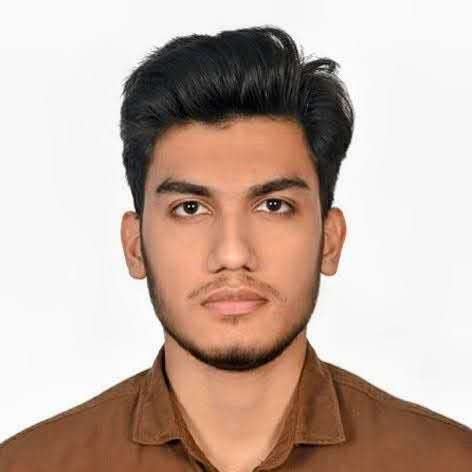
\includegraphics[width = 3.8cm]{Headshot_image}}; 
\end{tikzpicture}
    \hfill\vline\hfill
\end{minipage}
\begin{minipage}[c]{0.60\textwidth}
    \vspace{4pt} % Adjust this value for padding ABOVE the name
    \textbf{\Huge \scshape{Md. Sohanuzzaman Shanto}} \\[4pt] % Adjust this value for padding BELOW the name
    \small Rajshahi, Bangladesh \\
    \small +880 1774 786 111 \\
    \small \href{mailto:md.sohanuzzaman@proton.me}{\underline{md.sohanuzzaman@proton.me}} \\
    \small \href{https://linkedin.com/in/sohanuzzaman3301}{\underline{linkedin.com/in/sohanuzzaman3301}} \\
    \small \href{https://sohanuzzaman3301.github.io}{\underline{sohanuzzaman3301.github.io}} \\
\end{minipage}

%-----SUMMARY - Tech Support focused -
\section{Summary}
  \begin{itemize}[leftmargin=0.5cm, label={}]
    \small{\item{Google IT Support Certified fresher with self-taught Linux daily user — troubleshooting Windows/Linux, networking (TCP/IP, DNS, DHCP) and Active Directory. Lab-based ticketing, remote diagnosis and customer support. Bilingual Bengali/English, available immediately, shift-ready for Rajshahi/Dhaka/Remote.}}
  \end{itemize}

%-----EDUCATION - STEP 2 -----------------------------------------------------
\section{Education}
  \CVSubHeadingListStart
    \CVSubheading
      {{Bachelor of Engineering $|$ \emph{\small{Computer Science and Technology}}}}{Feb. 2022 -- Jan. 2026}
      {Wuhan Institute of Technology}{Wuhan, China}
      \CVItemListStart
        \CVItem{Graduated Jan 2026 — First-Class Scholarship for Academic Excellence (Ranked 1st in batch, 2025)}
      \CVItemListEnd
  \CVSubHeadingListEnd

%-----SKILLS - Tech Support focused (ATS keywords) -------------------------
\section{Technical Skills}
  \begin{itemize}[leftmargin=0.5cm, label={}]
     \small{\item{
      \textbf{IT Support \& Troubleshooting}{: Windows, Linux, Active Directory, Microsoft 365, Hardware/Software Troubleshooting, Remote Support (AnyDesk/TeamViewer), Ticketing \& Customer Service} \\
      \textbf{Networking \& Systems}{: TCP/IP, DNS, DHCP, OSI Model, Routing \& Switching, Wireshark, Nmap, System Administration} \\
      \textbf{Tools \& Scripting}{: Python, Bash, SQL, Wazuh dashboards, Splunk (SPL), Elastic (KQL)} \\
     }}
  \end{itemize}

%-----CERTIFICATIONS - Tech Support set (5) ---------------
\section{Certifications (Selected)}
  \CVSubHeadingListStart
    \item
      \begin{tabular*}{0.97\textwidth}{l@{\extracolsep{\fill}}r}
        \textbf{Google IT Support Professional Certificate} \textit{\small(Google / Coursera $|$ Jan 2026)} & \href{https://www.credly.com/badges/98cc58ec-2e39-4863-938f-b5c895a6dcb8/public_url}{\small Verify} \\
      \end{tabular*}
    \item
      \begin{tabular*}{0.97\textwidth}{l@{\extracolsep{\fill}}r}
        \textbf{The Bits and Bytes of Computer Networking} \textit{\small(Google / Coursera $|$ Dec 2025)} & \href{https://coursera.org/account/accomplishments/records/8LUX3EMPI9OJ}{\small Verify} \\
      \end{tabular*}
    \item
      \begin{tabular*}{0.97\textwidth}{l@{\extracolsep{\fill}}r}
        \textbf{Operating Systems and You: Becoming a Power User} \textit{\small(Google / Coursera $|$ Jan 2026)} & \href{https://coursera.org/account/accomplishments/records/40S2OH9S895Z}{\small Verify} \\
      \end{tabular*}
    \item
      \begin{tabular*}{0.97\textwidth}{l@{\extracolsep{\fill}}r}
        \textbf{System Administration and IT Infrastructure Services} \textit{\small(Google / Coursera $|$ Jan 2026)} & \href{https://coursera.org/account/accomplishments/records/ZHWJNSWXRKWI}{\small Verify} \\
      \end{tabular*}
    \item
      \begin{tabular*}{0.97\textwidth}{l@{\extracolsep{\fill}}r}
        \textbf{IT Security: Defense against the digital dark arts} \textit{\small(Google / Coursera $|$ Dec 2025)} & \href{https://coursera.org/account/accomplishments/records/0WYDGPH4VCM4}{\small Verify} \\
      \end{tabular*}
  \CVSubHeadingListEnd

%-----PROJECTS - Tech Support framed (user wording) ------------------------
\section{Projects \& Lab Experience}
  \CVSubHeadingListStart
    \CVSubheading
      {{Multi-Platform System Monitoring \& Troubleshooting Lab} $|$ \emph{\small{Wazuh, Suricata, Sysmon, VirtualBox, Kali Linux}}}{2026}
      {\href{https://github.com/Sohanuzzaman3301/SIEM_Home_Lab}{\underline{GitHub}}}{}
      \CVItemListStart
        \CVItem{Architected 3-VM lab (Windows Server, Linux, Kali) on NAT networks; diagnosed and resolved DNS, DHCP, TCP/IP failures to ensure cross-platform connectivity and uptime}
        \CVItem{Deployed centralized logging and real-time alerting; authored 20+ troubleshooting runbooks for recurring anomalies, standardizing resolution and reducing investigation time}
      \CVItemListEnd
    \CVSubheading
      {{Web Infrastructure \& Reverse-Proxy Access Lab} $|$ \emph{\small{SafeLine WAF, DVWA, Nginx, Kali Linux}}}{2026}
      {\href{https://github.com/Sohanuzzaman3301/safeline-waf-homelab}{\underline{GitHub}}}{}
      \CVItemListStart
        \CVItem{Deployed reverse-proxy infra for backend apps; troubleshot HTTP/HTTPS, SSL/TLS and upstream failures to maintain availability and validate access paths}
        \CVItem{Configured rate-limiting and access-control via log analysis; documented exceptions and workflows in knowledge base for rapid team reference}
      \CVItemListEnd
  \CVSubHeadingListEnd

%-----EXPERIENCE - STEP 6 (compact) ----------------------------------------
\section{Experience}
  \CVSubHeadingListStart
    \CVSubheading
      {Freelance Flutter Developer}{Jun. 2024 -- Feb. 2025}
      {Independent Contractor}{Remote}
      \CVItemListStart
        \CVItem{Built Flutter apps with Firebase Auth/Firestore (least-privilege) — client delivery \& async support}
      \CVItemListEnd
  \CVSubHeadingListEnd

%-----LANGUAGES - STEP 7 ---------------------------------------------------
\section{Languages}
  \begin{itemize}[leftmargin=0.5cm, label={}]
     \small{\item{\textbf{English} — C1 (TOEFL 103/120) $|$ \textbf{Bengali} — Native (Bangla)}}
  \end{itemize}

\end{document}
